\lecture{13}{9 April.}{}
\begin{eg}
    Suppose \(f(x) = \frac{1}{x^2}\) is defined on \(\mathbb{R}\), then we can extend it to \(f: \mathbb{R} \to \mathbb{R} ^*\) so that 
    \[
        f(x) = \begin{dcases}
            \frac{1}{x^2}, &\text{ if } x \neq 0 ;\\
            \infty , &\text{ if } x = 0.
        \end{dcases}
    \]   
    Then \(f\) is measurable. Note that if we define \(f\) by \(f: \Omega \to \mathbb{R}\), then \(f^{-1} ((a, \infty]) = f^{-1} ((a, \infty))\) for all \(a \in \mathbb{R}\).     
\end{eg}

\begin{lemma}
    Let \(\Omega \subseteq \mathbb{R} ^n\) be measurable. For each positive integer \(n\), let \(f_n : \Omega \to \mathbb{R} ^*\) be a measurable function. Then, \(\sup _{n \in \mathbb{N}} f_n, \inf_{n \in \mathbb{N}} f_n, \limsup_{n \to \infty} f_n, \liminf_{n \to \infty} f_n \) are measurable. In particular, if \(\lim_{n \to \infty} f_n(x) = f(x) \) for \(f: \Omega \to \mathbb{R} ^*\), then \(f\) is also measurable.    
\end{lemma}

\begin{proof}
    Let \(g(x) = \sup _{n \in \mathbb{N}} f_n(x)\), then \(g\) is measurable iff \(g^{-1}((a,\infty ])\) is measurable for any \(a \in \mathbb{R}\). Also,
    \begin{align*}
        x \in g^{-1}((a, \infty]) &\iff g(x) > a \iff \sup_{n \in \mathbb{N}} f_n(x) > a  \iff \exists k \in \mathbb{N} \text{ s.t. } f_k(x) > a \\
        & \iff \exists k \in \mathbb{N} \text{ s.t. } x \in f_k^{-1}((a, \infty]) \iff x \in \bigcup_{n=1}^{\infty} f_n^{-1}((a, \infty]). 
    \end{align*}    
    Hence, \(g^{-1} ((a, \infty]) = \bigcup_{n=1}^{\infty} f_n^{-1}((a,\infty]) \), so it sufficies to show that \(\bigcup_{n=1}^{\infty} f_n^{-1}((a, \infty]) \) is measurable. However, since for all \(n \in \mathbb{N}\), \(f_n\) is measurable, so \(f_n^{-1}((a, \infty])\) is measurable, and thus we're done. 

    Let \(h(x) = \inf _{n \in \mathbb{N}} f_n(x)\), then \(h\) is measurable iff \(h^{-1}((a, \infty])\) is measurable for all \(a \in \mathbb{R}\). Now since 
    \begin{align*}
        x \in h^{-1}((a, \infty]) &\iff h(x) \in (a, \infty] \iff \inf_{n \in \mathbb{N}} f_n(x) \in (a, \infty] \iff \inf _{n \in \mathbb{N} } f_n(x) > a \iff \forall n \in \mathbb{N}, \ f_n(x) > a \\
        &\iff \forall n \in \mathbb{N} , \ f_n(x) \in (a, \infty] \iff \forall n \in \mathbb{N} , \ x \in f_n^{-1}((a, \infty]) \iff x \in \bigcap_{n=1}^{\infty} f_n^{-1}((a, \infty]).
    \end{align*}         
    Hence, \(h^{-1}((a, \infty]) = \bigcap_{n=1}^{\infty} f_n^{-1}((a, \infty])\). However, since for all \(n \in \mathbb{N}\), \(f_n\) is measurable, so \(f_n^{-1}((a, \infty])\) is measurable, and thus we're done.

    Now we define \(g_N(x) = \sup _{n \ge N} f_n(x)\), then we know \(g_N\) is measurable for all \(N \in \mathbb{N}\) by what we've proved. Now since 
    \[
        \limsup_{n \to \infty} f_n(x) = \lim_{n \to \infty} \sup _{k \ge n} f_k(x) = \inf _{N \ge 1} \sup _{n \ge N} f_n(x) = \inf_{N \ge 1} g_N(x),  
    \]  
    so by what we've proved, we know \(\inf_{N \ge 1} g_N(x)\) is measurable, and we;re done. 

    Similar argument can be used to prove \(\liminf_{n \to \infty} f_n(x) \) is measurable.

\end{proof}

\chapter{Lebesgue Integration}


\section{What is Lebesgue integration?}

Lebesgue integration is a way of defining the integral of a function by grouping together points that have \emph{similar output values}. Instead of cutting the \emph{$x$-axis} into many thin intervals, as in Riemann integration, Lebesgue integration studies the sets of points where the function lies in certain value ranges and measures the size of those sets.

Informally, the two viewpoints are:
\begin{itemize}[leftmargin=1.5em]
    \item \textbf{Riemann integration:} slice the domain into vertical strips and add ``width $\times$ height.''
    \item \textbf{Lebesgue integration:} slice the range into horizontal bands and add ``value $\times$ measure of the set having that value.''
\end{itemize}

This change of perspective makes Lebesgue integration much more flexible. It can integrate many functions that are badly behaved from the Riemann point of view, and it works especially well in probability, Fourier analysis, and modern analysis.

\section*{The main idea}

Suppose a function $f$ takes the value approximately $y$ on a set of points whose length is approximately $m$. Then its contribution to the integral is approximately
\[
y \cdot m.
\]
Adding these contributions over all output levels leads to the Lebesgue integral.

For nonnegative functions, one can think of the construction as approximating $f$ by step functions built from \emph{horizontal} layers. In this way, the Lebesgue integral measures area by organizing the graph according to function values rather than according to input intervals.

\section*{How is it different from Riemann integration?}

The essential difference is the direction of the partition.

\begin{center}
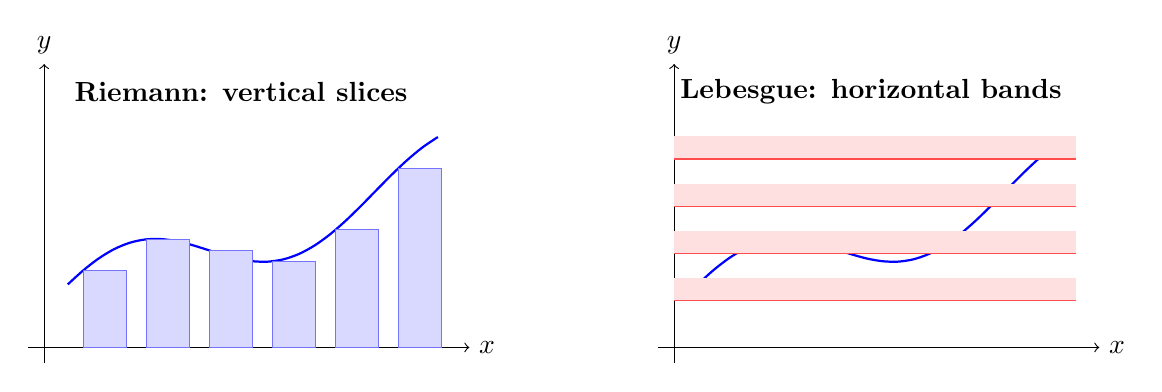
\begin{tikzpicture}[scale=1.0]
    % Left panel: Riemann
    \draw[->] (-0.2,0) -- (5.4,0) node[right] {$x$};
    \draw[->] (0,-0.2) -- (0,3.6) node[above] {$y$};
    \node at (2.5,3.25) {\textbf{Riemann: vertical slices}};

    \draw[domain=0.3:5,smooth,variable=\x,thick,blue] plot ({\x},{0.5 + 0.35*\x + 0.45*sin(deg(1.5*\x))});

    \foreach \x in {0.5,1.3,2.1,2.9,3.7,4.5} {
        \pgfmathsetmacro{\h}{0.5 + 0.35*\x + 0.45*sin(deg(1.5*\x))}
        \filldraw[fill=blue!15,draw=blue!55] (\x,0) rectangle +(0.55,\h);
    }

    % Right panel: Lebesgue
    \begin{scope}[xshift=8cm]
        \draw[->] (-0.2,0) -- (5.4,0) node[right] {$x$};
        \draw[->] (0,-0.2) -- (0,3.6) node[above] {$y$};
        \node at (2.5,3.25) {\textbf{Lebesgue: horizontal bands}};

        \draw[domain=0.3:5,smooth,variable=\x,thick,blue] plot ({\x},{0.5 + 0.35*\x + 0.45*sin(deg(1.5*\x))});

        \foreach \y in {0.6,1.2,1.8,2.4} {
            \draw[red!70, thick] (0,\y) -- (5.1,\y);
            \fill[red!12] (0,\y) rectangle (5.1,{\y+0.28});
        }
    \end{scope}
\end{tikzpicture}
\end{center}

\begin{itemize}[leftmargin=1.5em]
    \item In \textbf{Riemann integration}, the interval on the $x$-axis is divided into many small subintervals. One samples the function in each interval and sums rectangle areas.
    \item In \textbf{Lebesgue integration}, the $y$-axis is divided into small bands. For each band, one looks at all $x$ such that $f(x)$ falls inside that band, then measures how large that set is.
\end{itemize}

So Riemann organizes the area by \emph{where the input lies}, while Lebesgue organizes it by \emph{what values the function takes}.

\section*{Why Lebesgue integration is more powerful}

Lebesgue integration handles limits of functions much better. For example, if a sequence of functions converges in a reasonable way, the Lebesgue integral often allows us to interchange limit and integral. This is one of the main reasons it became the standard notion of integration in advanced mathematics.

It also integrates some functions that are not Riemann integrable. The classical example is the Dirichlet function on $[0,1]$:
\[
f(x)=
\begin{cases}
1, & x \in \mathbb{Q},\\
0, & x \notin \mathbb{Q}.
\end{cases}
\]

This function is discontinuous at every point, so it is not Riemann integrable. However, the rational numbers in $[0,1]$ have Lebesgue measure $0$, so from the Lebesgue point of view the function is equal to $0$ almost everywhere. Therefore,
\[
\int_0^1 f(x)\,dx = 0
\]
in the Lebesgue sense.

\section*{A visual example}

The next picture shows the Dirichlet function schematically. The dense blue points near $y=1$ represent rational inputs, and the dense red points near $y=0$ represent irrational inputs. Since the rational set has measure zero, the upper layer contributes no area in the Lebesgue sense.

\begin{center}
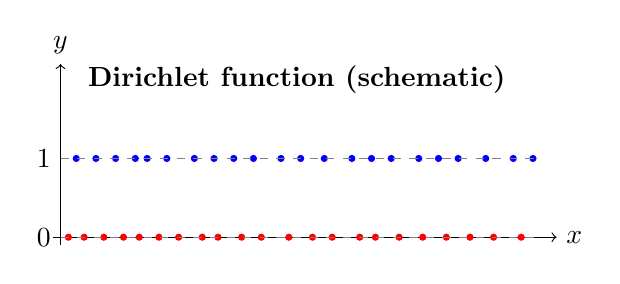
\begin{tikzpicture}[scale=1.0]
    \draw[->] (-0.1,0) -- (6.3,0) node[right] {$x$};
    \draw[->] (0,-0.1) -- (0,2.2) node[above] {$y$};
    \node at (3,2.0) {\textbf{Dirichlet function (schematic)}};
    \node[left] at (0,1) {$1$};
    \node[left] at (0,0) {$0$};

    \foreach \x in {0.2,0.45,0.7,0.95,1.1,1.35,1.7,1.95,2.2,2.45,2.8,3.05,3.35,3.7,3.95,4.2,4.55,4.8,5.05,5.4,5.75,6.0} {
        \fill[blue] (\x,1) circle (1.3pt);
    }

    \foreach \x in {0.1,0.3,0.55,0.8,1.0,1.25,1.5,1.8,2.0,2.3,2.55,2.9,3.2,3.45,3.8,4.0,4.3,4.6,4.9,5.2,5.5,5.85} {
        \fill[red] (\x,0) circle (1.3pt);
    }

    \draw[dashed, gray] (0,1) -- (6.1,1);
    \draw[dashed, gray] (0,0) -- (6.1,0);
\end{tikzpicture}
\end{center}

\section*{Summary}

\begin{itemize}[leftmargin=1.5em]
    \item \textbf{Riemann integration} partitions the domain and adds areas of vertical rectangles.
    \item \textbf{Lebesgue integration} partitions the range and measures the size of the sets where the function takes certain values.
    \item Lebesgue integration is better suited to complicated functions and to taking limits.
    \item Every Riemann integrable function is Lebesgue integrable, but not every Lebesgue integrable function is Riemann integrable.
\end{itemize}

In short, Lebesgue integration is a more robust and more powerful notion of area, built to handle modern analysis.

\newpage

\begin{definition}
    Let \(\Omega \subseteq \mathbb{R} ^n\) be a measurable set, and let \(f: \Omega \to \mathbb{R}\) be a measurable function. We say \(f\) is a simple function if the image of \(f(\Omega)\) is finite, i.e. \(\exists c_1, \dots , c_N\) s.t. for any \(c \in \Omega\), \(f(x) = c_j\) for some \(1 \le j \le N\).        
\end{definition}

\begin{eg}
    Let \(\Omega \subseteq \mathbb{R} ^n\) be a measurable set, and let \(E\) be a measurable subset of \(\Omega\). Define the characteristic function \(\chi _E: \Omega \to \mathbb{R}\) by 
    \[
        \chi _E (x) = \begin{dcases}
            1, &\text{ if } x \in E ;\\
            0, &\text{ if } x \in \Omega \setminus E.
        \end{dcases}
    \]    
    Then, we claim that \(\chi _E\) is measurable. Note that 
    \[
        \chi _E^{-1}(I) = \begin{dcases}
            \varnothing , &\text{ if } 0 \notin I, 1 \notin I ;\\
            E, &\text{ if } 0 \notin I, 1 \in I ;\\
            \Omega \setminus E, &\text{ if } 0 \in I, 1 \notin I ;\\
            \Omega , &\text{ if } 0 \in I, 1 \in I.
        \end{dcases}
    \] 
\end{eg}

\begin{lemma}
    Let \(\Omega \subseteq \mathbb{R} ^n\) be measurable, and let \(f: \Omega \to \mathbb{R}\) and \(g: \Omega \to \mathbb{R}\) be simple function. Then, \(f + g\) is also simple and for any \(c \in \mathbb{R}\), the function \(cf\) is also simple.      
\end{lemma}

\begin{proof}
    Suppose \(f(\Omega) = \left\{ a_1, \dots , a_N \right\} \) and \(g(\Omega) = \left\{ b_1, \dots , b_M \right\} \), then \((f + g)(\Omega) = \left\{ a_i + b_j \right\}_{\substack{1 \le i \le N \\ 1 \le j \le M}} \), which is finite, so \(f + g\) is simple. 

    Also, \((cf)(\Omega) = \left\{ ca_1, \dots , ca_N \right\} \), which is also finite, so \(cf\) is simple.      
\end{proof}

\begin{lemma}
    Let \(\Omega \subseteq \mathbb{R} ^n\) be measurable, and let \(f: \Omega \to \mathbb{R}\) be a simple function. Then, there exists finitely many distinct real numbers \(c_1, \dots , c_N\) and finitely many pairwise disjoint measurable sets \(E_1, \dots , E_N \subseteq \Omega\) s.t. \(f = \sum_{j=1}^N c_j \chi _{E_j} \).     
\end{lemma}

\begin{proof}
    Suppose \(f(\Omega ) = \left\{ c_1, \dots , c_N \right\} \), where \(c_i \neq c_j\) for all \(i \neq j\). Define \(E_j = f^{-1} (\left\{ c_j \right\} )\) for each \(1 \le j \le N\), then \(\left( E_j \right)_{j=1}^N \) are pairwise disjoint. Since \(f(x) = c_{\ell } \) for some \(1 \le \ell \le N\) for all \(x \in \Omega\), \(\Omega = \bigcup_{j=1}^{N} E_j \). Note that 
    \[
        E_j = f^{-1} (\left\{ c_j \right\} ) = \bigcap_{k=1}^{\infty} f^{-1} \left( \left( c_j - \frac{1}{k}, c_j + \frac{1}{k} \right)  \right),  
    \]       
    then since \(f\) is measurable, we know \(E_j\) is measurable. Now for \(x \in \Omega\), we know \(x \in E_k\) for some \(1 \le k \le N\). Hence, \(f(x) = c_k\), and thus 
    \[
        \sum_{j=1}^N c_j \chi _{E_j} (x) = c_k \chi _{E_k} (x) = c_k = f(x). 
    \]      
    Thus, \(f = \sum_{j=1}^N c_j \chi _{E_j} \). 
\end{proof}

\begin{lemma}
    Let \(\Omega \subseteq \mathbb{R} ^n\) be measurable, and let \(f: \Omega \to [0, \infty]\) be a measurable function. Then there exists a sequence of simple functions \(\left\{ f_n \right\}_{n=1}^{\infty}  \) with \(f_n: \Omega \to \mathbb{R}\) s.t. each \(f_n \ge 0\), and the sequence is increasing:
    \[
        0 \le f_1(x) \le f_2(x) \le \dots \quad \text{ for all } x \in \Omega, 
    \]     
    and \(\lim_{n \to \infty} f_n(x) = f(x) \) for all \(x \in \Omega\).  
\end{lemma}

\begin{proof}
    For each integer \(n \ge 1\), define 
    \[
        E_{n, k} \coloneqq \left\{ x \in \Omega: \frac{k}{2^n} \le f(x) < \frac{k+1}{2^n} \right\}, \quad k = 0, 1, \dots , n 2^n - 1,
    \] 
    and \(F_n \coloneqq \left\{ x \in \Omega: f(x) \ge n \right\} \). Then define 
    \[
        f_n(x) \coloneqq \sum_{k=0}^{n 2^n - 1} \frac{k}{2^n} \chi _{E_{n, k}} (x) + n \chi_{F_n}(x).
    \]
    Thus, \(f_n\) is obtained from \(f\) by truncating at height \(n\) and then rounding down to the nearest multiple of \(2^{-n}\). Note that If \(f(x) < n\), then \(\exists 0 \le k \le n2^n - 1\) s.t.
    \[
        \frac{k}{2^n} \le f(x) < \frac{k+1}{2^n},
    \]      
    so \(f_n(x) = \frac{k}{2^n}\), and if \(f(x) \ge n\), then \(f_n(x) = n\). 

    Now we try to write down the explicit formula for \(f_n\). Fix \(x \in \Omega \), then write \(a \coloneqq f(x) \in [0, \infty]\).

    \begin{claim}
        \[
            f_n(x) = \min \left( n, \frac{\lfloor 2^n a \rfloor}{2^n} \right) = \min \left( n, \frac{\lfloor 2^n f(x) \rfloor}{2^n} \right).   
        \]
    \end{claim}
    \begin{explanation}
        If \(a = f(x) \ge n\), then \(f_n(x) = n\), and \(n \le \frac{\lfloor 2^n f(x) \rfloor}{2^n}\), so this is true. If \(a = f(x) < n\), then \(\exists 0 \le k \le n 2^n - 1\) s.t. 
        \[
            \frac{k}{2^n} \le a < \frac{k + 1}{2^n} \iff k \le 2^n a < k + 1,
        \]     
        so \(k = \lfloor 2^n a \rfloor\). Since \(f(x) \in E_{n, k}\), we have 
        \[
            f_n(x) = \frac{k}{2^n} = \frac{\lfloor 2^n a \rfloor}{2^n}.
        \] 
        Thus, in this case, \(f_n(x) = \min \left( n, \frac{\lfloor 2^n a \rfloor}{2^n} \right) \).  

    \end{explanation}   

    By this claim, we know =\(0 \le f_n(x) \le f(x)\) for all \(n\).

    Now we show \(f_n(x) \le f_{n+1}(x)\). 
    \begin{itemize}
        \item Case 1: \(n \le f(x)\), then \(f_n(x) = n\), and \(f_{n+1}(x) = \min \left( n+1, \frac{\lfloor 2^{n+1} f(x) \rfloor}{2^{n+1}} \right) \ge n\), so we're done. 
        \item Case 2: \(f(x) < n\), then 
        \[
            f_n(x) = \min \left( n, \frac{\lfloor 2^n f(x) \rfloor}{2^n} \right) = \frac{\lfloor 2^n f(x) \rfloor}{2^n}. 
        \]
        Thus, \(\exists \) unique \(m = \lfloor 2^n f(x) \rfloor \le 2^n f(x) < m + 1\), and 
        \[
            f_{n+1}(x) = \min \left( n+1, \frac{\lfloor 2^{n+1} f(x) \rfloor}{2^{n+1}} \right), 
        \]  
        and note that 
        \[
            2m \le 2^{n+1}f(x) < 2(m + 1),
        \]
        so 
        \[
            f_n(x) = \frac{\lfloor 2^n f(x) \rfloor}{2^n} = \frac{m}{2^n} = \frac{2m}{2^{n+1}} \le \frac{\lfloor 2^{n+1} f(x) \rfloor}{2^{n+1}} = f_{n+1}(x),
        \]
        where the last equality holds since \(f(x) < n < n + 1\). 
    \end{itemize} 

\end{proof}
